\documentclass[a4paper,12pt]{article}

\usepackage[english,brazilian]{babel}
\usepackage[utf8]{inputenc}
\usepackage{icomma}
\usepackage{amsmath}
\usepackage{makecell}
\usepackage{graphicx}
\usepackage{fancyhdr}
\usepackage{url}
\renewcommand{\baselinestretch}{1.5}
\usepackage{titling}
\usepackage{geometry}
\usepackage{subfigure}
\geometry{
 a4paper,
 left=35mm,
 right=15mm,
 top=1in,
 bottom=1in,
}
\usepackage{amsmath}
\usepackage{amssymb}
\usepackage{subfigure}
\usepackage{multirow}
\usepackage[table]{xcolor}
\usepackage[backend=bibtex,style=ieee,sorting=none]{biblatex}
\usepackage{algorithm}
\usepackage[noend]{algpseudocode}
\usepackage{float}
\usepackage{pdfpages}
\usepackage{enumerate}
\bibliography{main}
\newcolumntype{C}{>{\centering\arraybackslash}p{1em}}


\newpage

\begin{document}
\selectlanguage{brazilian}

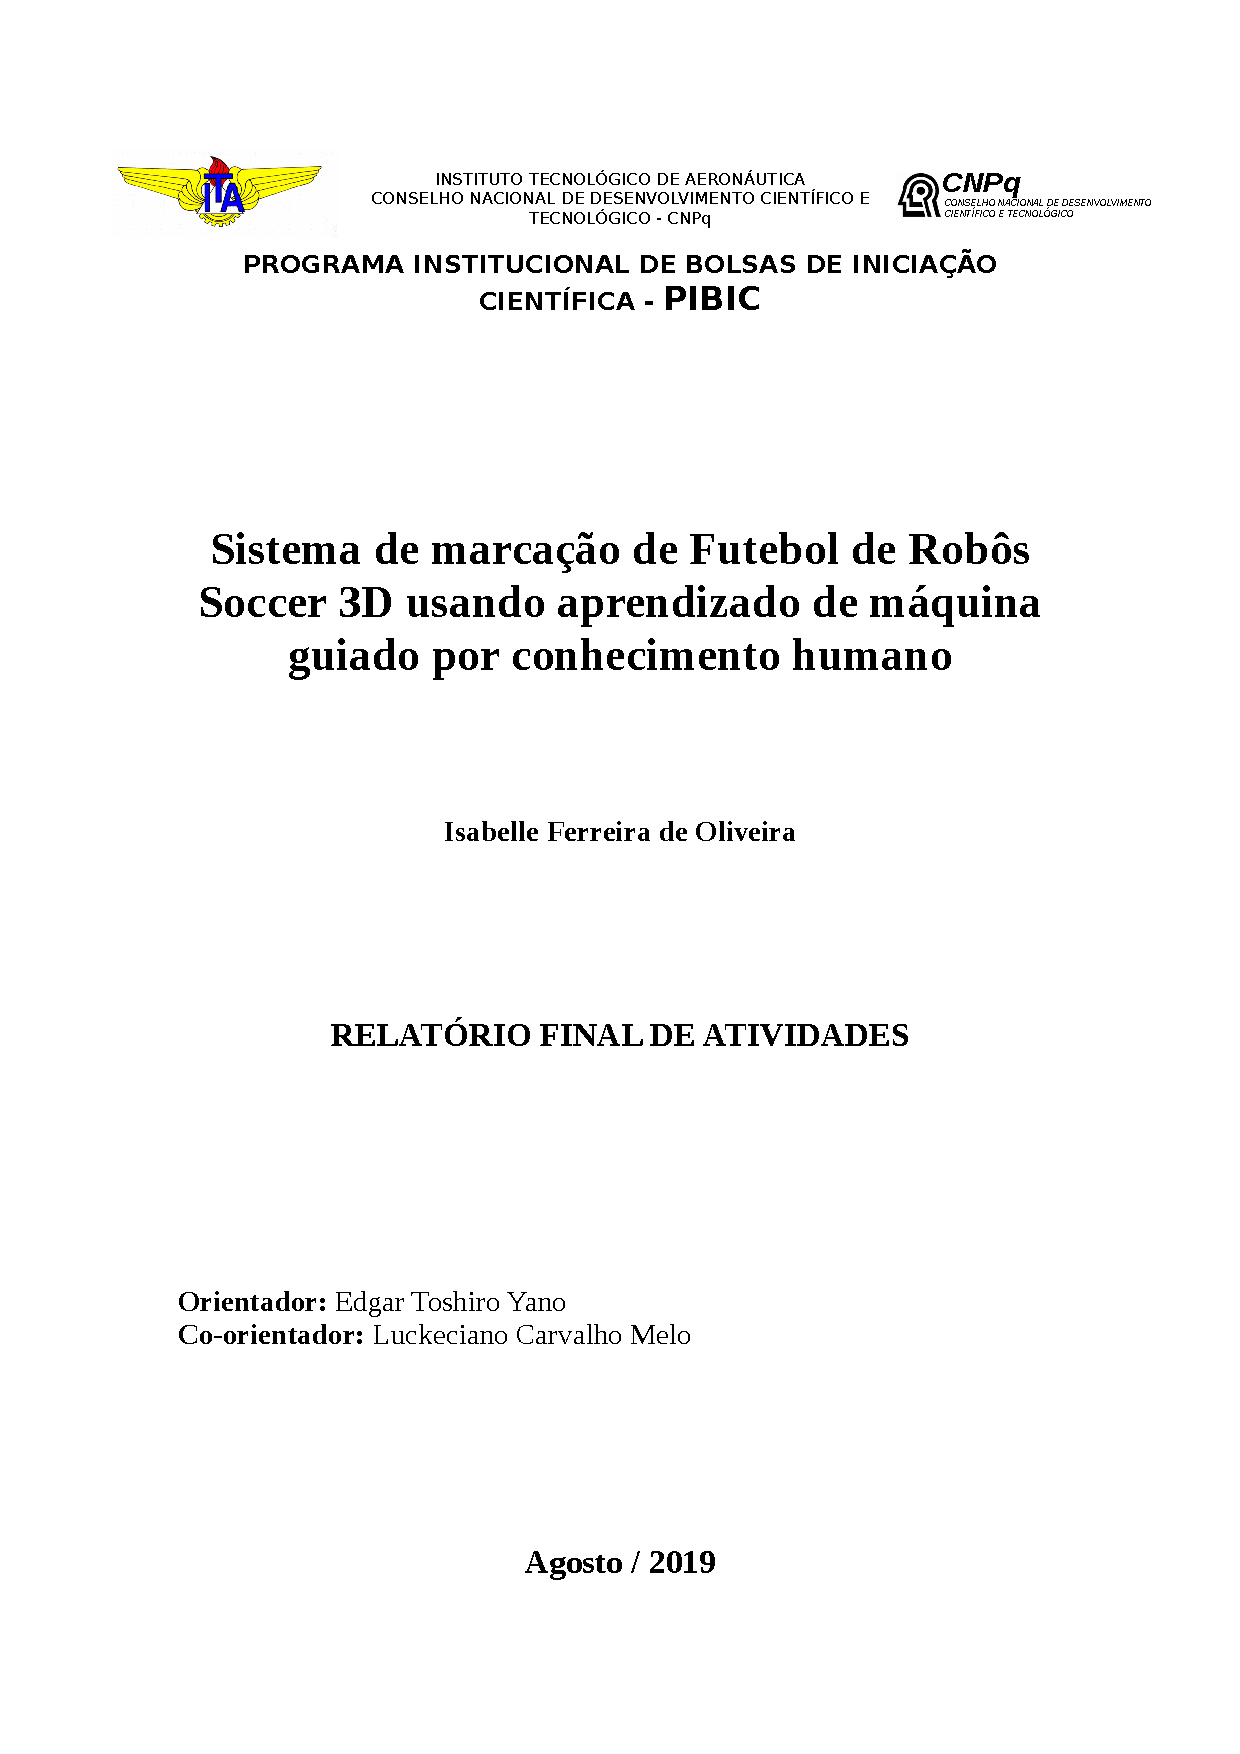
\includepdf[pages={1-},scale=1]{Inicio.pdf}


\tableofcontents

\newpage

\section{Resumo do Plano Inicial}
\label{secao:plano_inicial}

O objetivo deste trabalho é desenvolver e implementar uma inteligência por meio de rede neural que determine quais oponentes devem ser marcados em um determinado momento de partida futebol de robôs humanóides simulados. A confecção das entradas iniciais da rede neural será realizada por conhecimento humano, com o auxílio de uma interface gráfica que permita interagir com os frames da partida. 

O contexto é uma partida de futebol segundo a RoboCup, competição de robótica anual internacional, categoria Soccer Simulation 3D (Soccer3D). A partir da posição dos robôs oponentes e da bola, deve-se obter quais jogadores adversários deveriam ou não ser marcados a fim de se evitar levar gols. Visa-se utilizar os resultados aqui alcançados pela equipe da ITAndroids, que representa o ITA, em competições nacionais e internacionais, como na competição Latin America Robotics Competition (LARC)/CBR e na própria RoboCup.

Planejamento Atualizado:
\begin{itemize}

\item 1o Bimestre (ago / set): Estudo dos critérios para marcação de oponentes e estudo de algoritmo de aprendizado de máquina.

\item 2o Bimestre (out / nov): Estudo de linguagem de ferramenta de interface gráfica e início da implementação da ferramenta de geração de dataset para a inteligência.

\item 3o Bimestre (dez / jan): Conclusão da implementação da ferramenta da geração de dataset para a inteligência e confecção do relatório parcial.

\item 4o Bimestre (fev / mar): Geração de amostras para a inteligência através da ferramenta gráfica, seleção da estrutura a ser usada na rede neural e implementação inicial, além de primeira análise dos resultados e alteração estrutural da rede caso necessário.

\item 5o Bimestre (abr / mai): Aprimoração dos resultados da inteligência através de novos dados de entrada, testes da rede para um dataset de teste no qual se tem uma resposta esperada e alterações finais estruturais para a rede após análise dos novos resultados.

\item 6o Bimestre (jun / jul): Análise final dos resultados, análise das melhorias do time com a nova estratégia de marcação, confecção do relatório final e redação do artigo para o ENCITA.

\end{itemize}

\section{Resumo das Atividades Realizadas}
\label{secao:atividades_realizadas}

Ao longo dos dois primeiros meses, foram realizados estudos sobre como a marcação era feita atualmente na equipe ITAndroids e qual seriam os algoritmos de aprendizado de máquina utilizados. O método utilizado se baseava em algumas condições heurísticas referentes aos oponentes.

Foi decidido inicialmente que será usado um algoritmo supervisionado de classificação. Esse algoritmo foi escolhido entre as opções de algortimos supervisionados de regressão, algoritmos não supervisionados e algoritmos de reforço. Uma introdução a esse assuntos pode ser encontrada em [1]. Uma descrição sobre porque seria o ideal entre essas opções aplicar um algoritmo supervisionado de classificação está apresentada na seção 4.

Ao longo do segundo bimestre, estudou-se quais linguagens se usaria para a ferramenta de inferface gráfica. Entre Java e Qt em C++, preferiu-se a última opção, tendo em vista que todo o restante de código da equipe ITAndroids está escrito em C++, inclusive outras ferramentas de interfaces gráficas, facilitando a integração e o suporte técnico. Para fins de simplificação do projeto, escolheu-se também utilizar de arquivos de texto (.txt) para armazenar os dados referentes às posições dos jogadores, oponentes e bola em campo, que serviriam de entrada para a inteligência. Dessa forma, nesse período foi iniciada a implementação da interface.

No terceiro bimestre, continuou-se a implementação da interface, codificando a lógica de leitura e escrita dos arquivos de texto (.txt), além do desenho do campo e dos jogadores e bola na tela. Já no quarto e quinto bimestres, concluiu-se a interface e se iniciou a geração de dados para entrada da inteligência. Esses dados foram produzidos a partir de frames reais de partidas de futebol simulado, em uma frequência de um frame a cada 30 segundos. Os times utilizados foram o ITAndroids Soccer 3D e o BahiaRT.

Por fim, no sexto bimestre, a rede neural de aprendizado supervionado foi desenvolvida. A linguagem escolhida foi Python, utilizando a framework Keras, devido sua ampla documentação online.

\section{Descrição do Problema}
\label{secao:enunciado_problema}

O sistema de marcação é um processo seqüencial usado para marcar jogadores oponentes que estão ofensivamente perigosos durante a partida. No contexto do futebol de robôs humanóides simulados, a marcação de oponentes pode ser muito crucial em uma partida, melhorando significantemente a defesa de um time. A marcação consiste no fato de se implementar um algoritmo que consiga utilizar o planejamento de trajetórias do robô de forma a dificultar que oponentes em situações de vantagem façam gols. Isso traz um desafio: decidir quais jogadores adversários estão em situação mais privilegiada em um determinado instante e deveriam ser marcados por agentes aliados. 

Nesse projeto, trabalhou-se com os robôs da competição Soccer Simulation 3D (Soccer3D): uma competição que robôs humanóides competem uns contra os outros em uma simulação realista das regras e da física de um jogo de futebol [2]. Cada time tem 11 jogadores: um goleiro e outros 10 que podem assumir posições dinâmicas, como zagueiro, atacante, etc., a critério de escolha de estratégia das equipes. A Figura \ref{fig:soccer3d-play} mostra uma cena de partida de Soccer3D (nesse exemplo, com apenas 9 jogadores em cada time).

\begin{figure}[H]
	\centering
	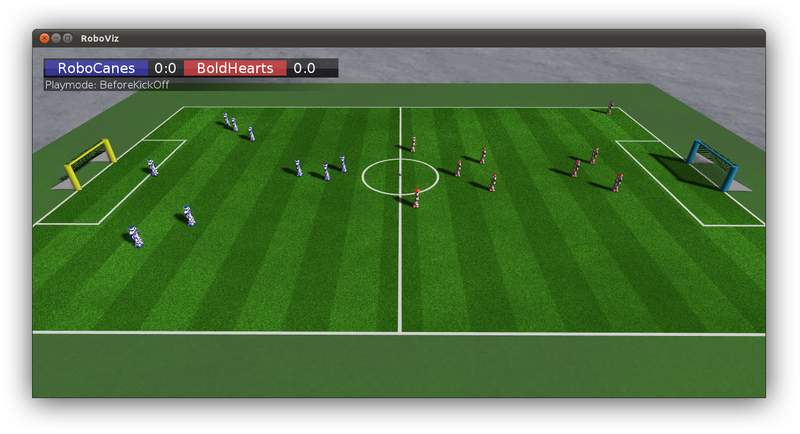
\includegraphics[width=0.8\textwidth]{figures/soccer3d-play.png}
   \caption{Um frame de uma partida de futebol simulado Soccer3D de 9 vs 9 jogadores [2].} \label{fig:soccer3d-play}
\end{figure}

As dimensões do campo de futebol são de 30 por 20 metros. Além disso, o campo é cercado por uma borda de 10 metros nas dimensões x e y, e o espaço além dessa área não é acessível para os jogadores. Uma representação do campo pode ser vista na Figura \ref{fig:soccer3d_field}.

\begin{figure}[H]
	\centering
	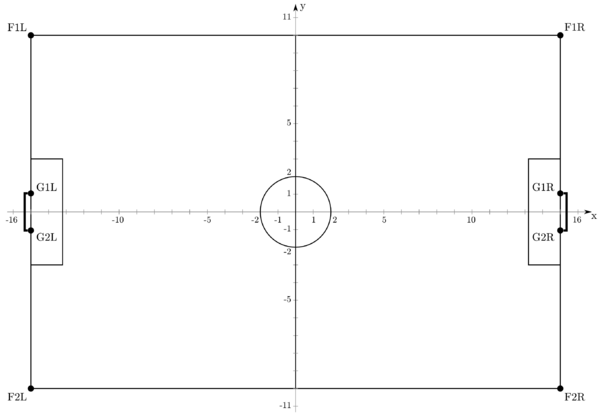
\includegraphics[width=0.5\textwidth]{figures/soccer3d-field.png}
   \caption{Representação de um campo de futebol simulado para partidas de Soccer3D [2].} \label{fig:soccer3d_field}
\end{figure}

O modelo atual de robô utilizado nas competições é baseado no robô \textit{Nao}, da empresa \textit{Aldebaran Robotics}, apresentado na Figura \ref{fig:nao_robot}. Esse robô possui 22 articulações para controlar o movimento de seu corpo, uma câmera direcional com campo de visão de 120 graus de largura na cabeça, e cabeça que pode girar em dois graus de liberdade, variando de -120 a 120 graus da esquerda para a direita e de -45 a 45 graus de baixo para cima [3].

\begin{figure}[H]
	\centering
	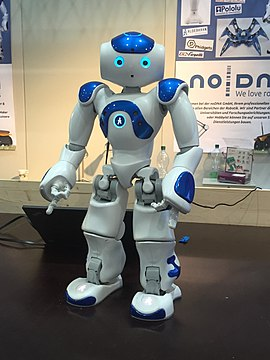
\includegraphics[width=0.3\textwidth]{figures/nao-robot.jpg}
   \caption{Robô \textit{Nao}, da empresa \textit{Aldebaran Robotics} [3].} \label{fig:nao_robot}
\end{figure}

As regras completas podem ser lidas em [4]\cite{cbr2008}.

A competição utiliza o simulador \textit{Simspark} [5] e o servidor \textit{Rcsserver3D} [6] para simular tanto a física, quanto a partida entre os multiagentes robóticos. Os times (computadores \textit{clients}) se conectam ao computador servidor (\textit{server}) através de um \textit{agentproxy} chamdo \textit{MagmaProxy} [7]. Os jogos são executados em \textit{Ubuntu 16.04} de 64 Bits e são exebidos na ferramenta de visualização e monitoramento \textit{Roboviz} (\textit{monitor}) [8]. A Figura \ref{fig:computers-schema} a seguir mostra o esquema dessa comunicação.

\begin{figure}[H]
	\centering
	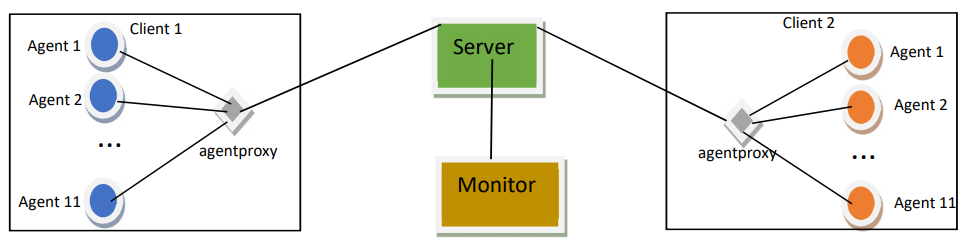
\includegraphics[width=0.9\textwidth]{figures/computers-schema.png}
   \caption{Representação de como o software e hardware do ambiente da competição são utilizados. Existem dois computadores \textit{clients}, um para cada equipe, chamados \textit{client1} e \textit{client2}; um servidor; e um computador monitor (\textit{Roboviz}) [4].} \label{fig:computers-schema}
\end{figure}

A linguagem utilizada para o projeto da equipe ITAndroids foi C++, pois é uma linguagem que tem uma velocidade de execução alta e tem boa escalabilidade para um projeto grande.

Nesse contexto, surgem várias questões a serem resolvidas para se ter um time vencedor. Nesse projeto, será abordado o seguinte problema: dada as posições dos jogadores oponentes e da bola, deve-se escolher quais adversários são os mais ofensivamente perigosos e deveriam ser marcados.

Grande parte do projeto se trata da ferramenta de interface gráfica que vai captar o conhecimento humano e formar o dataset da inteligência artificial. O intuito é fazer um compilado das ideias inconscientes acerca de quais oponentes deveriam ser marcados, para posteriormente automatizar o processo por meio da inteligência artificial, indo além das condições heurísticas utilizadas atualmente. Para resolver esse problema, então, foi feito a interface em Qt de C++.

A outra parte essencial é o desenvolvimento da inteligência artificial. Ela que vai lidar com o compilado de ideias captados pela interface anteriormente, a fim de automatizar a marcação de adversários durante a partida.

\section{Resultados Obtidos}

Nessa seção, serão apresentados os resultados obtidos do estudo do problema, desde como está a sendo resolvido atualmente pela equipe até uma ideia inicial de substituir a atual resolução do problema por uma com aprendizado de máquina na tomada de decisão para o sistema de marcação pra robôs jogadores de futebol Soccer3D. Além disso, foi explicado a lógica da implementação da ferramenta de interface gráfica.

\subsection{Sistema de Marcação Atual}

Atualmente na ITAndroids [9], o sistema de marcação é responsável por decidir os jogadores que serão marcados, definir as funções para marcar esses jogadores e, por fim, usa o sistema de Atribuição de Funções (\textit{Role Assignment}) para designar agentes aliados para essas funções definidas.

No primeiro momento, para decidir quais oponentes serão marcados, um método heurístico é atualmente usado com base nas seguintes condições sobre o oponente, isto é, marca-se o oponente caso ele:

\begin{itemize}
\item Esteja perto o suficiente para dar um chute a gol;
\item Não seja o adversário mais próximo da bola;
\item Não esteja muito perto da bola;
\item Não esteja muito longe atrás da bola.
\end{itemize}

Depois disso, um conjunto de agentes do time aliado é selecionado para marcar os adversários escolhidos. Para isso, as posições onde os agentes aliados ficarão para marcar os oponentes são calculadas como 1,5 metros contados a partir do o oponente marcado, na reta que o conecta ao centro do gol do time aliado. Um esquema do dessa regra está exposto na Figura \ref{fig:marking-position}.

\begin{figure}[H]
	\centering
	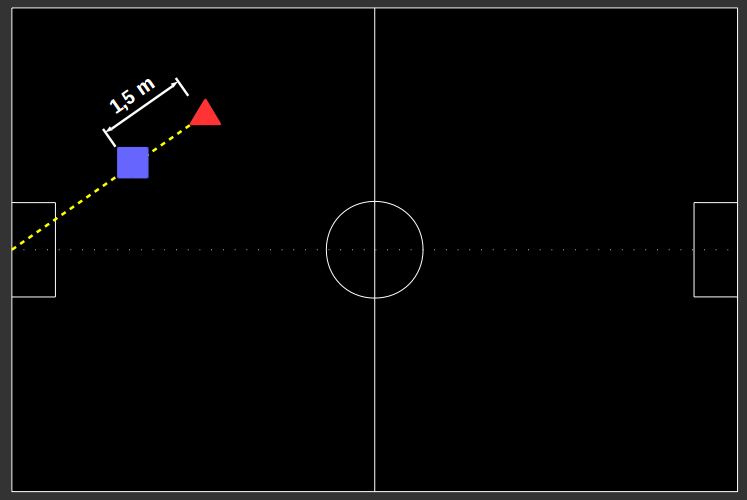
\includegraphics[width=0.6\textwidth]{figures/marking-position.png}
   \caption{Esquema de como é escolhido a posição de marcação (quadrado azul) para um determinado oponente a ser marcado (representado em triângulo vermelho). O lado esquerdo do campo é o do time aliado.} \label{fig:marking-position}
\end{figure}

As posições de formação naturais a serem substituídas por posições de marcação são as mais próximas de cada posição de marcação, e sua seleção é feita usando o algoritmo húngaro, que calcula a soma mínima de distâncias entre as posições de formação anteriores e as posições de marcação.

\subsection{Ferramenta de Interface Gráfica}
\subsubsection{Arquivo de texto (.txt)}
Os arquivos estão em um diretório próprio chamado /positions para fins de organização e são nomeados como frameX.txt, no qual X é o número do frame ao qual esse arquivo se refere. Dentro dos arquivos, é seguido o padrão apresentado na Figura \ref{fig:frame1-txt}.

\begin{figure}[H]
	\centering
	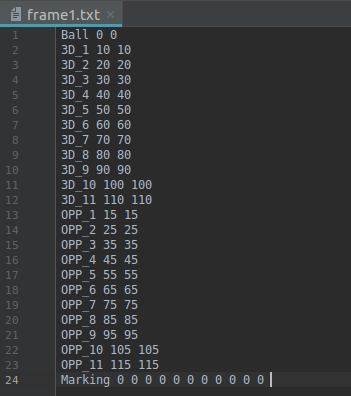
\includegraphics[width=0.4\textwidth]{figures/frame1-txt.png}
   \caption{Exemplo de arquivo de texto (.txt) que servia de entrada e saída da interface gráfica. Na figura, está apresentada o frame1.txt.} \label{fig:frame1-txt}
\end{figure}

No arquivo, cada linha se inicia com uma palavra indentificadora, que pode ser Ball, 3D\underline{\space}i, OPP\underline{\space}j e Marking, no qual i e j são os números do agente aliado e do oponente em questão, respectivamente.

Os números após os indentificadores Ball, 3D\underline{\space}i e 3D\underline{\space}j são respectivamente as coordenadas x e y da bola, dos agentes aliados e dos oponentes. Já na última linha, após o identificador Marking, existe 11 inteiros, que podem ser 0 ou 1, indicando se quais oponentes deverão ser marcados naquele frame (1 para marcado e 0 para não marcado).

\subsubsection{Classe Frame}
\textit{Frame} é a classe que guarda todas as informações dos agentes e bola em campo em um determinado frame.

Nessa classe, existe um vetor \textit{teammates}, um vetor \textit{opponents} e objeto \textit{ball}, referentes aos agentes aliados, aos jogadores adversários e à bola, respectivamente. Nesses atributos são guardados, por exemplo, suas coordenadas x e y, se determinado agente está ou não caído, se determinado oponente está ou não selecionado, etc.

Sua utilização se dá na classe principal da interface gráfica, na qual existe um vetor de Frames, responsável por manter as informações contidas em todos os frames documentados nos arquivos de texto, que já foram lidos pela classe PositioningFileManager.

\subsubsection{Classe PositioningFileManager}
\textit{PositioningFileManager} é o nome da classe que lida com a leitura e escrita dos arquivos de texto. Suas principais funções são \textit{populateFrame} e \textit{writeMarkingVector}.

\begin{itemize}
\item \textbf{\textit{populateFrame}:} lê o arquivo de texto e retorna um objeto da classe \textit{Frame} com os dados salvos nesse arquivo, como posições dos agentes em campo, da bola, e vetor de marcação naquele momento.

\item \textbf{\textit{writeMarkingVector}:} essa função é chamada ao botão confirm ser clicado. Ela recebe as marcações feitas pelo usuário na interface e reescreve o vetor após o indicativo \textit{Marking} no arquivo de texto referente àquele frame.
\end{itemize}

\subsubsection{Classe MarkingSystemWidget}
\textit{MarkingSystemWidget} é a classe principal da interface gráfica, que herda da \textit{QMainWindow}, da \textit{Framework Qt}.

Nessa classe, além de outros atributos referentes a detalhes mais internos, existe um vetor \textit{frames} (que guarda todos os frames criados pela classe \textit{PositioningFileManager} ao ler os arquivos da pasta /positions) e um inteiro \textit{currentFrame} (utilizado para que a interface saiba qual frame deve exibir em sua tela).

No construtor dessa classe também é criado todo o design da tela da interface. Essa tela possui os seguintes 4 botões:
\begin{itemize}
\item prevFrame;
\item nextFrame;
\item unmarkAll;
\item confirm.
\end{itemize}

Ao clicar nos botões prevFrame e nextFrame, a tela é atualizada para exibir os 22 jogadores e a bola nesse determinado frame selecionado. O botão unmarkAll desseleciona todos os oponentes que o usuário tinha selecionado para marcar naquele frame em questão. Por fim, o botão confirm chama a classe PositioningFileManager e escreve no arquivo de texto (.txt) quais os jogadores oponentes que deveriam ser marcados naquela situação de jogo.

Dessa forma, a aparência da interface está como representada nas Figuras \ref{fig:ms-widget} e \ref{fig:ms-widget2}.

\begin{figure}[H]
	\centering
	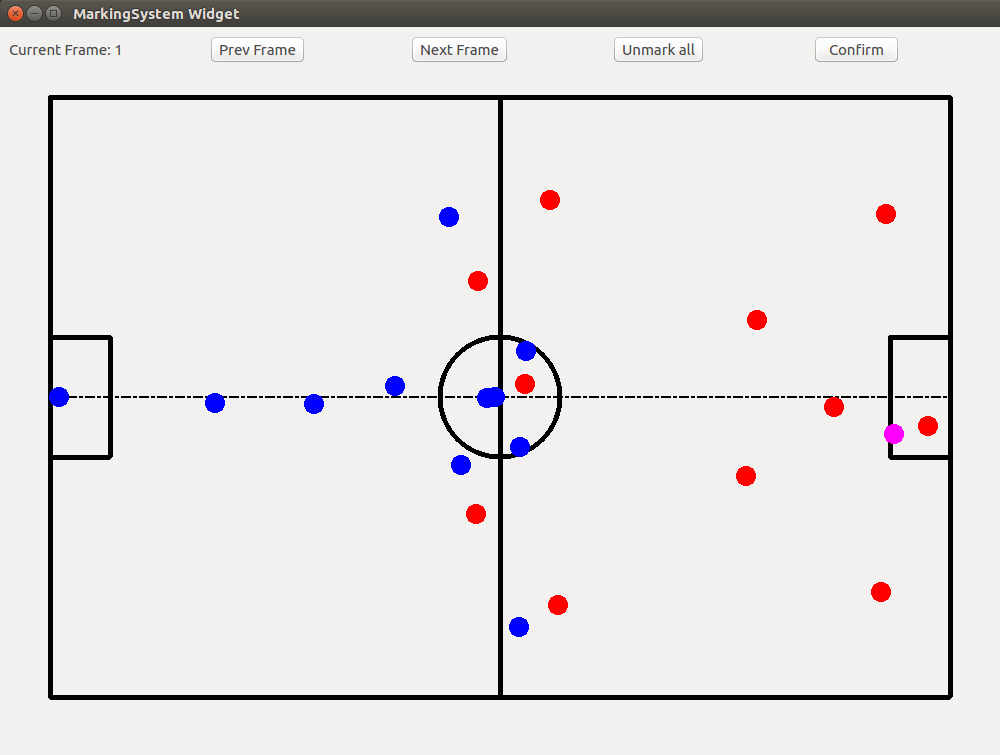
\includegraphics[width=0.7\textwidth]{figures/frame1.png}
   \caption{Aparência da ferramenta de interface gráfica Marking System Widget.} \label{fig:ms-widget}
\end{figure}

\begin{figure}[H]
	\centering
	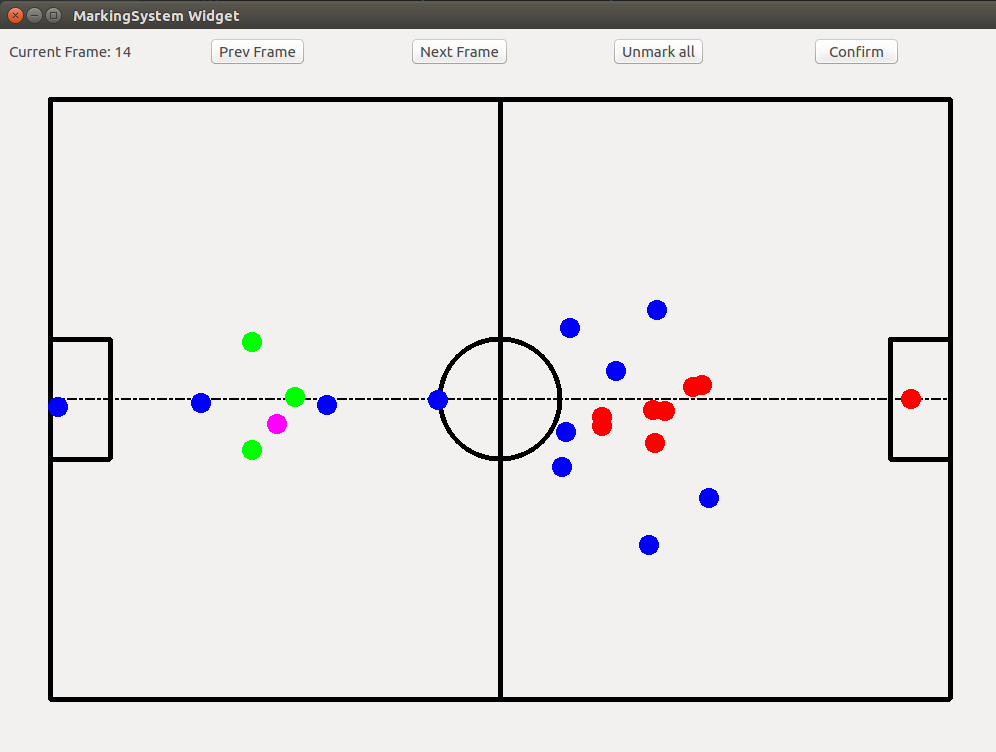
\includegraphics[width=0.7\textwidth]{figures/frame14.png}
   \caption{Aparência da ferramenta de interface gráfica Marking System Widget, com alguns oponentes marcados.} \label{fig:ms-widget2}
\end{figure}

\subsection{Algoritmo Supervisionado de Classificação}

\subsubsection{Escolha do algoritmo}

Aprendizado de máquina (ou \textit{Machine Learning}, em inglês), de forma simplificada, é um método de análise de dados que automatiza o processo de aprender a partir de dados de entrada, identificar padrões e tomar decisões com o mínimo de intervenção humana. Uma descrição mais detalhada dessa seção pode ser encontrada na referência [1].

Os métodos mais adotados de machine learning podem ser classificados em três grandes grupos, tendo em vista os tipos de dados de entrada da inteligência: aprendizado supervisionado, aprendizado não supervisionado ou  aprendizado por reforço. Em um aprendizado supervisionado, A inteligência tem acesso a informações como
entradas e saídas esperadas, aprendendo como se por através de um "professor". O objetivo do método é encontrar a função que leva das entradas às saídas.

Outra classificação possível se refere as diferentes saídas possíveis de sistemas de aprendizado de máquina: classificação, regressão ou clustering. Em um problema de classificação, as entradas são classificadas entre duas ou mais tipos discretos e a inteligência deve ser capaz de, para novas entradas (ainda sem classificação), vinculá-las a uma dessas classes pré-definidas. Um exemplo disso é classificar emails como sendo ou não spams, dadas as palavras utilizadas em seu texto.

No contexto do projeto de pesquisa, tem-se o objetivo de, partindo de um dataset com as posições dos 22 jogadores e da bola (além de qual é o lado aliado e qual o adversário) e o conhecimento humano de quais jogadores devem ser marcados, classificar cada um dos 11 oponentes de uma situação ainda não vista pela inteligência como marcáveis ou não. Tendo em vista o exposto acima, fica evidente em primeiro momento que o método de aprendizado de máquina supervisionado de classificação aparenta-se ser o ideal para se atingir o resultado esperado.

\subsubsection{Implementação da rede neural}

A implementação foi feita utilizando a framework Keras, em Python, de acordo com o resumo apresentado na Figura \ref{fig:network-summary}.

\begin{figure}[H]
	\centering
	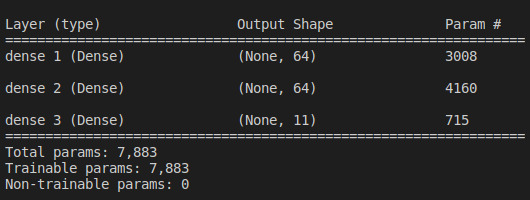
\includegraphics[width=0.5\textwidth]{figures/network_summary.jpeg}
   \caption{Resumo da rede neural implentada utilizando Keras, em Python.} \label{fig:network-summary}
\end{figure}

A rede consiste de 3 camadas escondidas: as duas primeiras com 64 neurônios e a última com 11 neurônios, referente as informações dos 11 jogadores oponentes (se eles devem ser marcados, ou não). A função de ativação utilizada foi a tangente hiperbólica para as duas primeiras camadas escondidas e sigmoide para a última, com learning rate de $10^{-5}$. Foram utilizadas um total de 5000 épocas. O conjunto completo de todos os hiperparâmetros utilizados foi apresentado na Figura \ref{fig:hiperparametros}.

\begin{figure}[H]
	\centering
	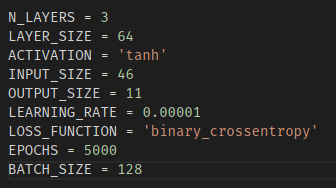
\includegraphics[width=0.4\textwidth]{figures/hiperparametros.png}
   \caption{Resumo dos hiperparâmetros utilizados na rede neural implentada.} \label{fig:hiperparametros}
\end{figure}

\subsubsection{Resultados da rede}

Utilizou-se inicialmente um dataset de 500 frames, referentes a mais de 4 horas seguidas de partida. Esse dataset foi gerado conforme explicado anteriormente, a partir de conhecimento humano. Desse conjunto de frames, 300 (60\% do total) foram escolhidos para o treinamento da rede, 100 (20\% do total) para set de validação cruzada. Já os últimos 100 (20\% do total), foram escolhidos para o teste propriamente dito, ou seja, um dataset no qual a rede jamais tinha tido contato anteriormente.

O treino da rede obteve um modelo com acurácia de 89.15\% no dataset de treino, 85.57\% no dataset de validação cruzada, e 86.92\% no dataset de teste. A evolução da acurácia e valor de custo com o passar das épocas foram apresentadas nas Figuras \ref{fig:acc} e \ref{fig:loss}.

\begin{figure}[H]
	\centering
	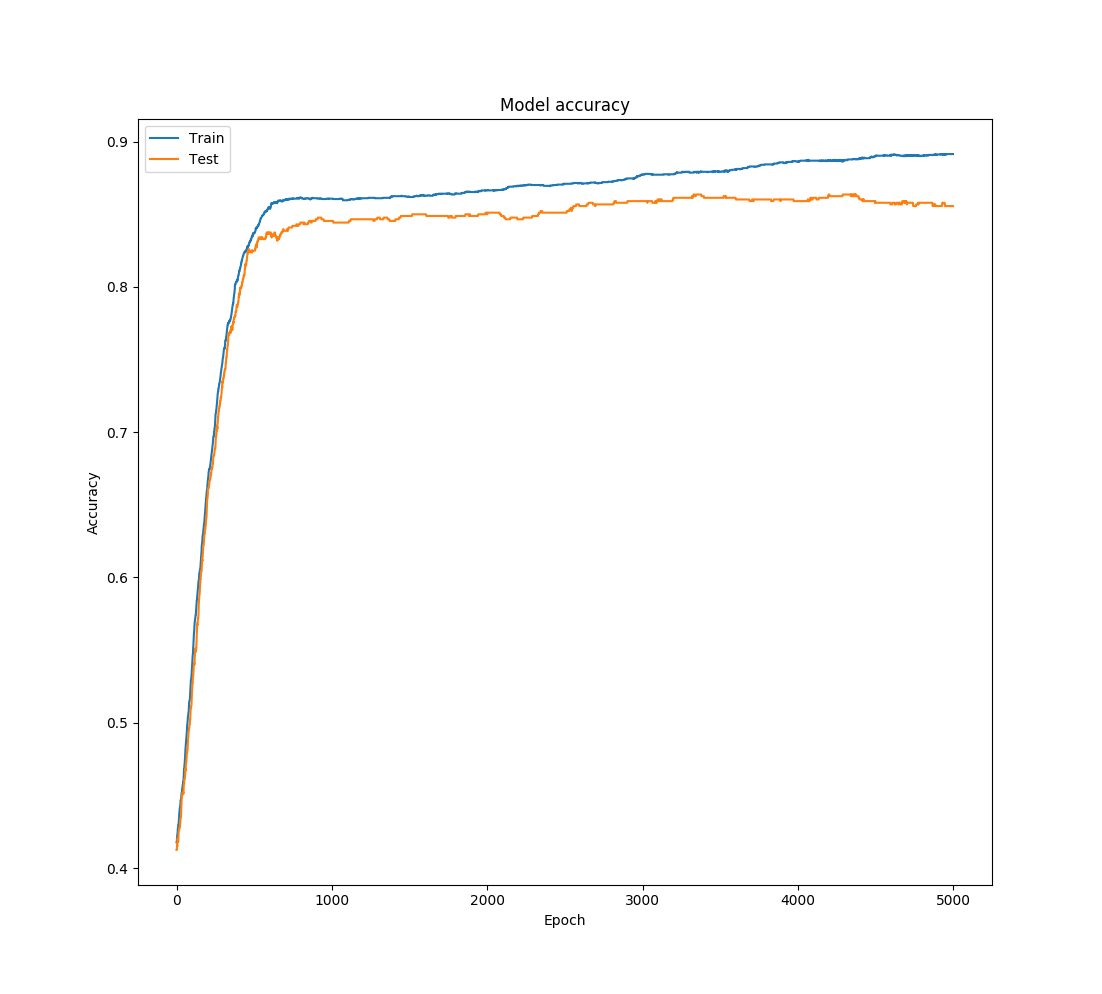
\includegraphics[width=0.6\textwidth]{figures/model_accuracy.png}
   \caption{Acurácia do modelo com o passar das épocas.} \label{fig:acc}
\end{figure}

\begin{figure}[H]
	\centering
	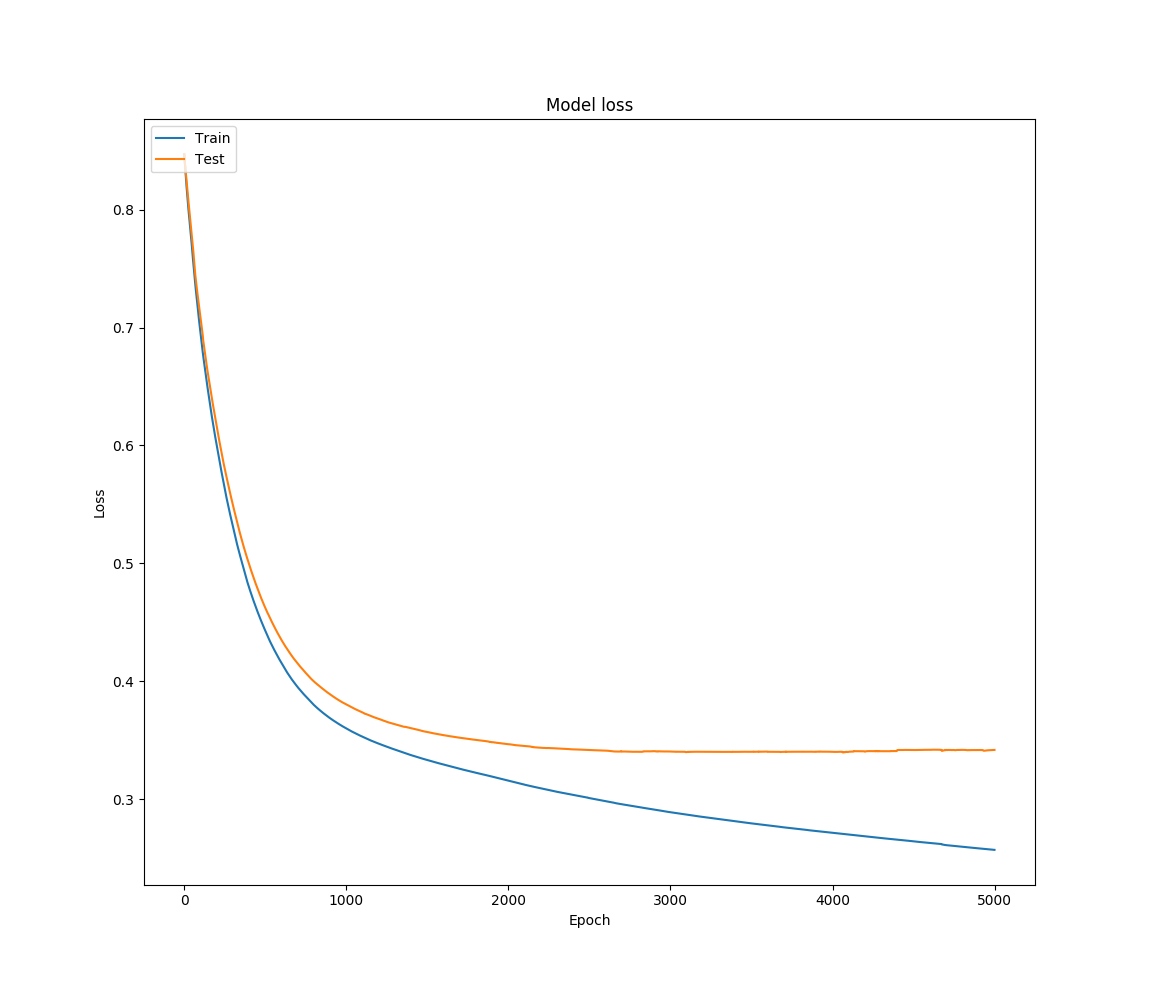
\includegraphics[width=0.6\textwidth]{figures/model_loss.png}
   \caption{Função de custo do modelo com o passar das épocas.} \label{fig:loss}
\end{figure}

Alguns exemplos dos resultados no dataset de teste foram apresentados a seguir.

Nas Figuras \ref{fig:frame507} e \ref{fig:frame459}, consegue-se perceber um funcionamento aceitável na escolha dos oponentes a serem marcados. Nota-se também que a rede desenvolveu uma tendência de se marcar poucos oponentes, o que não necessariamente é o desejado.

\begin{figure}[H]
	\centering
	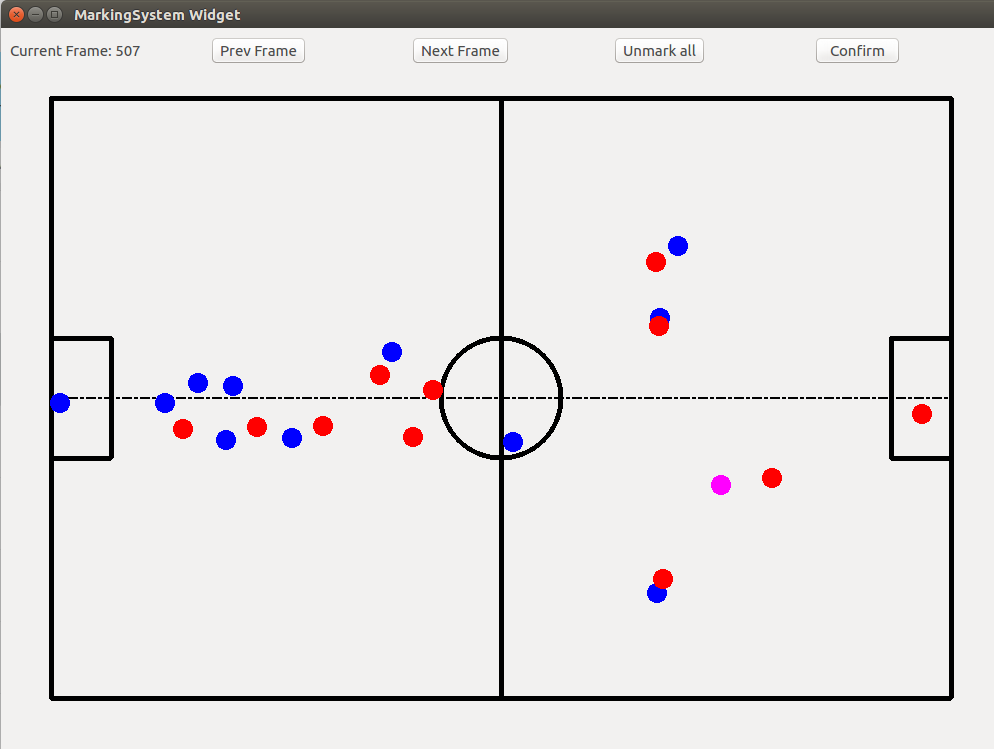
\includegraphics[width=0.6\textwidth]{figures/frame507.png}
   \caption{Exemplo de correta marcação. Para bola presente muito ao lado atacante do campo, é entendido que não se tem necessidade de marcar oponentes.} \label{fig:frame507}
\end{figure}

\begin{figure}[H]
	\centering
	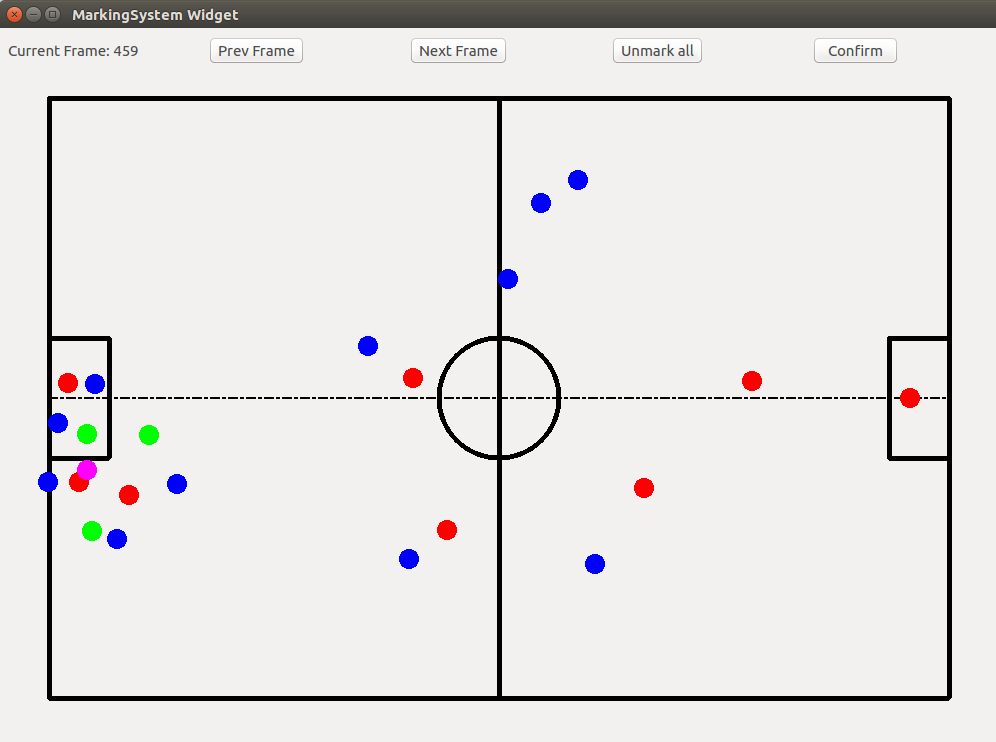
\includegraphics[width=0.6\textwidth]{figures/frame459.png}
   \caption{Exemplo de marcação satisfatória. Nota-se a tendência da rede de marcar poucos oponentes, uma vez que há outros oponentes em situação perigosa que não estão sendo marcados.} \label{fig:frame459}
\end{figure}

Na Figura \ref{fig:frame461}, por exemplo, pode-se perceber que essa escolha de se marcar poucos oponentes pode acabar sendo prejudicial em algumas situações reais de jogo.

\begin{figure}[H]
	\centering
	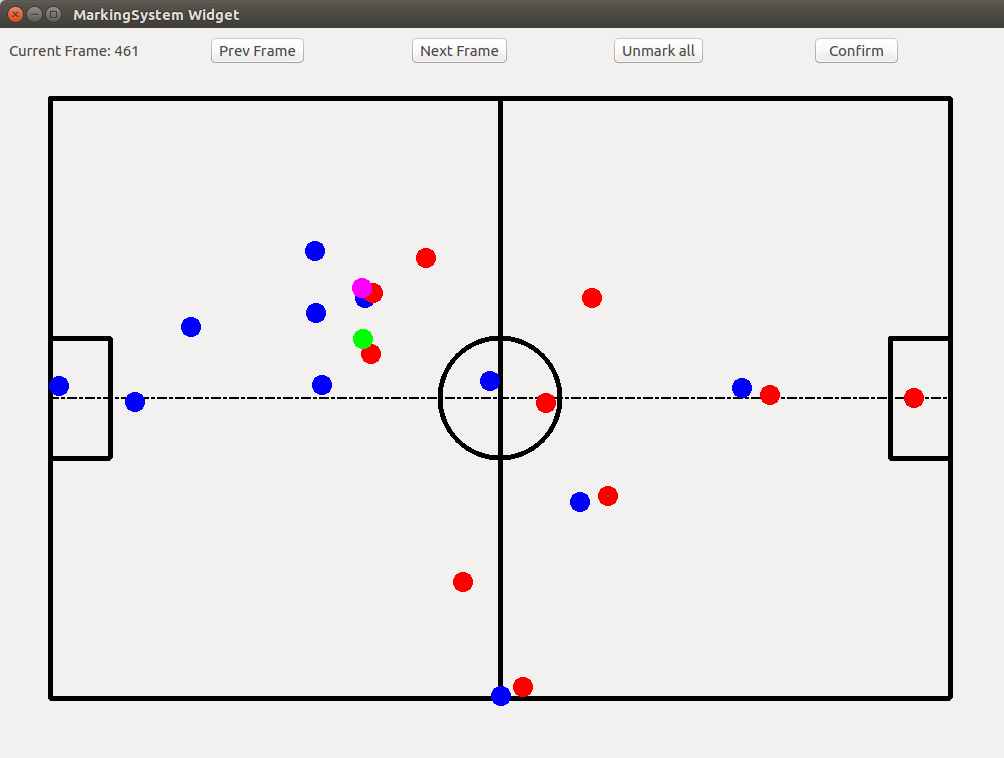
\includegraphics[width=0.6\textwidth]{figures/frame461.png}
   \caption{Exemplo de marcação não satisfatória, uma vez que apenas um oponente foi marcado, bastante próximo a outro também em posição perigosa.} \label{fig:frame461}
\end{figure}

\section{Conclusões}

O projeto de Iniciação Científica apresentou bons resultados, uma vez que a interface está em funcionamento, assim como as aquisições de conhecimento humano para geração de dados para a inteligência. Pode-se inclusive melhorar a inteligência, a partir da aquisição de mais dataset, por exemplo, ou revisão do atualmente desenvolvido. A forma como está atualmente implementado possibilita essa posterior melhoria, conforme se perceba a necessidade. Concomitantemente a isso, foi feita a seleção da estrutura a ser usada na rede neural e a sua implementação. Foi possível, também, analisar os resultados da estrutura implementada com os dados gerados pela interface, resultados esses que se mostraram satisfatórios.

\section{Agradecimentos}

\begin{itemize}
\item Ao CNPq, pelo apoio financeiro e motivacional.
\item À ITAndroids, equipe que representa o ITA na competição da LARC/CBR e Robocup, pela ideia do projeto, pela oportunidade de aplicação dos métodos estudados.
\item Ao professor Edgar Yano, meu orientador, e ao professor doutor Marcos Ricardo de Omena Máximo, co-orientador, ambos da Divisão da Ciência da Computação do ITA, pelo apoio nos estudos e no desenvolvimento do projeto.

\end{itemize}

\begin{thebibliography}{10}

\bibitem{ref1} E. Alpaydin, \textit{Introduction to machine learning}. MIT press, 2009.

\bibitem{ref2} S. Sourceforge, \textit{Soccer simulation}, \url{http://simspark.sourceforge.net/wiki/index.php/Soccer_Simulation}, [Online; acessado em 05-Janeiro-2019], 2012.

\bibitem{ref3} Wikipédia, \textit{Robocup 3d soccer simulation league: robot models}, \url{https://en.wikipedia.org/wiki/RoboCup_3D_Soccer_Simulation_League}, [Online; acessado em 05-Janeiro-2019], 2017.

\bibitem{ref4} RoboCup, \textit{Rules for the 2018 competition in montreal, canada}, \url{https://ssim.robocup.org/wp-content/uploads/2018/12/Rules_RoboCupSim3D2018.pdf}, [Online; acessado em 10-Janeiro-2019], 2018.

\bibitem{ref5} Sourceforge, \textit{Simspark}, \url{http://simspark.sourceforge.net/}, [Online; acessado em 15-Janeiro-2019].

\bibitem{ref6} RoboCup, \textit{The robocup soccer simulator}, \url{https://sourceforge.net/projects/sserver/}, [Online; acessado em 15-Janeiro-2019].

\bibitem{ref7} M. Offenburg, \textit{Magmaproxy},\url{https://github.com/magmaOffenburg/magmaProxy}, [Online; acessado em 17-Janeiro-2019].

\bibitem{ref8} M. Offenburg, \textit{Roboviz}, \url{https://github.com/magmaOffenburg/RoboViz}, [Online; acessado
em 20-Janeiro-2019].

\bibitem{ref9} ITAndroids, "Itandroids soccer3d team description paper 2019", \textit{RoboCup 2019}, vol.
2, p. 7, 2019.

%\bibitem{ref10} N. View, \textit{What is machine learning with sap}, \url{https://www.nextview.nl/what-is-machine-learning-with-sap/}, [Online; acessado em 20-Fevereiro-2019].

\end{thebibliography}

%\printbibliography


\end{document}